\documentclass[12pt,letterpaper]{article}
\usepackage[utf8]{inputenc}
\usepackage[spanish, english]{babel}
\usepackage{graphicx}
\usepackage{lettrine}
\usepackage{enumitem}
\usepackage[left=3cm,right=3cm,top=3cm,bottom=3cm]{geometry}
\usepackage{float} 
\usepackage{amsmath}
\usepackage{stackrel} 
\usepackage{multirow}
\usepackage{enumerate}
\renewcommand{\labelitemi}{$-$}
\renewcommand{\labelitemii}{$\cdot$}

\providecommand{\keywords}[1]
{
  \small	
  \textbf{\textit{Keywords: }} #1
}

\providecommand{\pclave}[1]
{
  \small	
  \textbf{\textit{Palabras Clave:}} #1
}
\begin{document}

\title{Caratula}
\begin{titlepage}
\begin{figure}[htb]
\begin{center}

\includegraphics[width=5cm]{./Imagenes/logo.png}
\end{center}
\end{figure}
\vspace*{-0.25in}
\begin{center}
\large{UNIVERSIDAD PRIVADA DE TACNA}\\
\vspace*{-0.025in}
INGENIERIA DE SISTEMAS  \\

\vspace*{0.5in}
\begin{large}
TITULO:\\
\end{large}

\vspace*{0.1in}
\begin{Large}
\textbf{TRABAJO ENCARGADO N° 01} \\
\end{Large}

\vspace*{0.3in}
\begin{Large}
\textbf{CURSO:} \\
\end{Large}

\vspace*{0.1in}
\begin{large}
BASE DE DATOS II\\
\end{large}

\vspace*{0.3in}
\begin{Large}
\textbf{DOCENTE:} \\
\end{Large}

\vspace*{0.1in}
\begin{large}
 Ing. Patrick Cuadros Quiroga\\
\end{large}

\vspace*{0.2in}
\vspace*{0.1in}
\begin{large}
Integrantes: \\
\begin{flushleft}
Sivirichi Falcón, Ricardo Alonso\hfill(2018060905) \\
Chambilla Maquera, Araceli Noemi\hfill(2018060897)\\
Alférez Ponce, Pedro Alberto\hfill(2020066317)\\
Cotrado Marino, Ana Luz\hfill(2018060907)\\

\end{flushleft}
\end{large}

\vspace*{0.1in}
\begin{large}
Tacna - Perú\\
2020
\end{large}
\end{center}

\end{titlepage}

\selectlanguage{spanish}
\begin{abstract}
El principal objetivo de este artículo es indagar sobre estructuras de datos y bases de datos relacionales para comprender la representación de la información en nuestro día a día.
La metodología utilizada fue el análisis y síntesis de la información proporcionada por diversos autores de libros y artículos. Como resultado, este artículo sintetiza un concepto claro sobre bases de datos relacionales y diversas estructuras de datos.
Este artículo concluye que las estructuras de datos son una colección, cuya organización se caracteriza por las funciones de acceso utilizadas para almacenar y acceder a elementos de datos individuales.
\end{abstract}
\pclave{estructura de datos, base de datos relacional.}

\begin{center}\rule{1\textwidth}{0.05mm} \end{center}

\selectlanguage{english}
\begin{abstract}
The main objective of this article is to investigate data structures and relational databases to understand the representation of information in our day to day.
The methodology used was the analysis and synthesis of the information provided by various authors of books and articles. As a result, this article synthesizes a clear concept about relational databases and various data structures.
This article concludes that data structures are a collection, the organization of which is characterized by the access functions used to store and access individual data elements.
\end{abstract}
\keywords{data structure, relational database.}

\selectlanguage{spanish}


\section{Introducción}
Cada día, la mayoría de nosotros nos encontramos con actividades que requieren algún tipo de interacción con una base de datos como el ingreso en un banco, reserva de una entrada, solicitud de una suscripción, compra de productos, etc. Estas interacciones son ejemplos de lo que se llama aplicaciones tradicionales de bases de datos, básicamente información numérica o de texto, aunque los avances tecnológicos también han permitido que existan nuevos tipos de información recolectable. La representación de la información es fundamental en ciencias de la computación y en informática, es por ello que el propósito principal de la mayoría de los programas de computadoras es almacenar y recuperar información, además de realizar cálculos. De modo práctico, los requisitos de almacenamiento y tiempo de ejecución exigen que tales programas deben organizar su información de un modo que soporte procesamiento eficiente.
Por estas razones, el estudio de estructuras de datos y de bases de datos relacional serán tratadas en este artículo. 

\section{Desarrollo}
\subsection{¿Qué es una base de datos relacional?}
Una base de datos relacional no es más que un modelo se utiliza en la actualidad para representar problemas reales y administrar datos de manera dinámica. Su principio fundamental consiste en el uso de  relaciones. Estas relaciones podrían considerarse en forma lógica como conjuntos de datos llamados tuplas.\cite{PEO2019}

\subsection{¿Qué es una estructura de datos?}
La estructura de datos está representada por una forma determinada que tenemos de organizar los datos de un equipo informático para que podamos utilizarlos de la manera más efectiva posible. Dependiendo del tipo de aplicación o recurso que vayamos a usar requerimos una estructura de datos independiente y distinta a las demás, dado que cada una encaja en el contexto de forma determinada y con una serie de objetivos.

\subsection{Principales tipos de estructuras:}
\subsubsection{Arrays:}
El arreglo es un tipo estructurado de datos, el cual es capaz de almacenar una colección de datos del mismo tipo y es la estructura de datos más utilizada por los programadores. También es la forma más simple de agrupar componentes de un mismo tipo y asociarlos a un número de orden de cada componente llamado í­ndice donde se almacenan en posiciones contiguas de memoria, además de poseer un tama ño. Además es una colección finita, homogénea y ordenada de elementos.
\begin{itemize}
\item Finita: Todo arreglo tiene un lí­mite; es decir, debe determinarse cuál será el número máximo de elementos que podrán formar parte del arreglo.
\item Homogénea: Esto significa que todos los elementos del arreglo deben ser del mismo tipo. (Todos enteros, todos reales, todos booleanos, etc.)
\item Ordenada: Se puede determinar cuál es el primer elemento, el segundo, el tercero,... y el n-ésimo elemento.
\end{itemize}
\begin{figure}[h]
\begin{center}
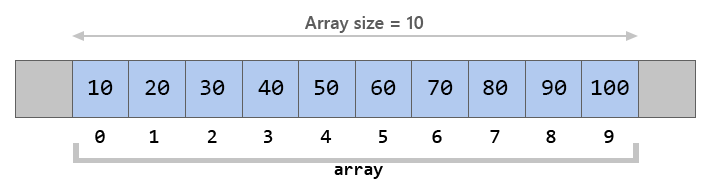
\includegraphics[width=12cm]{./Imagenes/array.png}
\caption{Representación gráfica de un array unidimensional.}
\label{rg1}
\end{center}
\end{figure}

\subsubsection{Listas Enlazadas:}
Secuencia ordenada de nodos donde cada nodo almacena: un dato (información), una referencia. Los nodos no tienen porqué estar contiguos en memoria. De esta manera los nodos pueden localizarse en cualquier parte de la memoria, utilizando la referencia que lo relaciona con otro nodo dentro de la estructura.
Las listas enlazadas permiten almacenar información en posiciones de memoria que no sean contiguas; y se almacena en los elementos nodos. Estos nodos poseen dos campos uno para almacenar la información o valor del elemento y otro para el enlace que determina la posición del siguiente elemento o nodo de la lista.
\begin{figure}[h]
\begin{center}
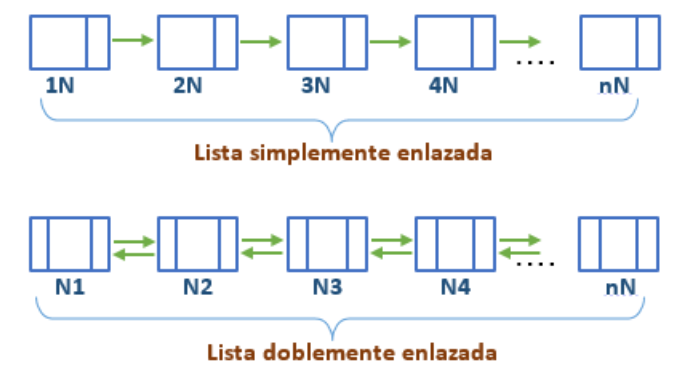
\includegraphics[width=9cm]{./Imagenes/listas.png}
\caption{Representación gráfica de listas enlazadas.}
\label{rg2}
\end{center}
\end{figure}
\vspace*{-0.4in}

\subsubsection{Pilas:}
Las pilas son estructuras de datos que tienen dos operaciones básicas: push (para insertar un elemento) y pop (para extraer un elemento). Su característica fundamental es que al extraer se obtiene siempre el último elemento que acaba de insertarse. Por esta razón también se conocen como estructuras de datos LIFO (del inglés Last In First Out).\\
Una posible implementación mediante listas enlazadas serí­a insertando y extrayendo siempre por el principio de la lista. Gracias a las pilas es posible el uso de la recursividad (lo veremos en detalle en el tema siguiente). La variable que llama al mismo procedimiento en el que está, habrá que guardarla así­ como el resto de variables de la nueva llamada, para a la vuelta de la recursividad ir sacandolas, esto es posible a la implementación de pilas. 
\begin{figure}[ht]
\begin{center}
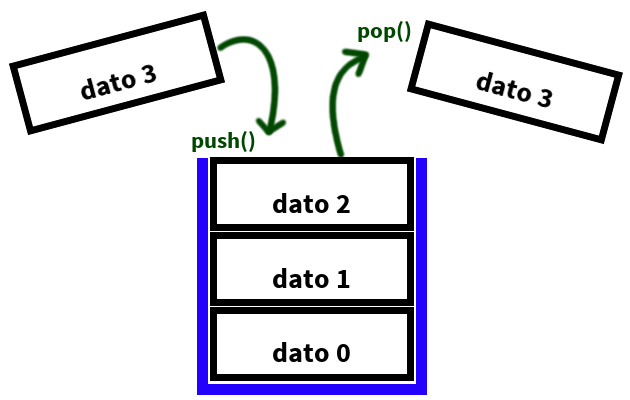
\includegraphics[width=6cm]{./Imagenes/pila.png}
\caption{Representación gráfica de una pila.}
\label{rg3}
\end{center}
\end{figure}

\subsubsection{Colas:}
Las colas también son llamadas FIFO (First In First Out), que quiere decir "el primero que entra es el primero que sale". 
\begin{itemize}
\item Colas simples: Se inserta por un sitio y se saca por otro, en el caso de la cola simple se inserta por el final y se saca por el principio. Para gestionar este tipo de cola hay que recordar siempre cual es el siguiente elemento que se va a leer y cual es el último elemento que se ha introducido. 
\item Colas circulares: En las colas circulares se considera que después del último  elemento se accede de nuevo al primero. De esta forma se reutilizan las posiciones extraí­das, el final de la cola es a su vez el principio, creándose un circuito cerrado.
\item Colas con prioridad: Las colas con prioridad se implementan mediante listas o arrays ordenados. No nos interesa en este caso que salgan en el orden de entrada sino con una prioridad que le asignemos. Puede darse el caso que existan varios elementos con la misma prioridad, en este caso saldrá primero aquel que primero llego (FIFO).
\end{itemize}
\vspace*{-0.2in}
\begin{figure}[h]
\begin{center}
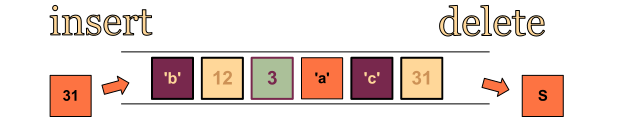
\includegraphics[width=10cm]{./Imagenes/cola.png}
\caption{Representación gráfica de una cola simple.}
\label{rg4}
\end{center}
\end{figure}
\vspace*{-0.4in}
\subsubsection{Arboles Binarios:}
Los árboles binarios son estructuras de datos muy similares a las listas doblemente enlazadas, en el sentido que tienen dos punteros que apuntan a otros elementos, pero no tienen una estructura lógica de tipo lineal o secuencial como aquellas, sino ramificada.  Tienen aspecto de árbol, de ahí­ su nombre.\\Un árbol binario es una estructura de datos no lineal en la que cada nodo puede apuntar a uno o máximo a dos nodos. También se suele dar una definición recursiva que indica que es una estructura compuesta por un dato y dos árboles. Esto son definiciones simples. Este tipo de árbol se caracteriza porque tienen un vértice principal y de él se desprenden dos ramas. La rama izquierda y la rama derecha a las que también se les conoce como subárboles.
\vspace*{-0.1in}
\begin{figure}[h]
\begin{center}
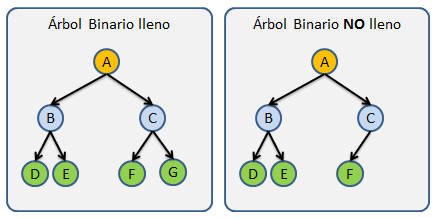
\includegraphics[width=7cm]{./Imagenes/arbolbinario.png}
\caption{Representación gráfica de arboles binarios.}
\label{rg5}
\end{center}
\end{figure}

\subsubsection{Grafos:}
Un grafo se define como un conjunto de vértices o nodos y un conjuntos de arcos. Se dice que hay un arco V1 y V2, que va del vértice al otro vértice cuando el nodo apunte al nodo V2. Un grafo se dice que no es dirigido si se cumple las condiciones de que un arco del grafo, entonces también lo que es el arco V2, V1.\\Para representarlo gráficamente se dibuja un conjunto de cí­rculos que simbolizan los vértices y un conjunto de segmentos entre ellos que representan los arcos. Si se trata de un arco dirigido los segmentos serán flechas. Un grafo valorado es aquel que tiene asociado un factor de peso, es decir aristas o arcos están ponderadas.
\vspace*{-0.1in}
\begin{figure}[h]
\begin{center}
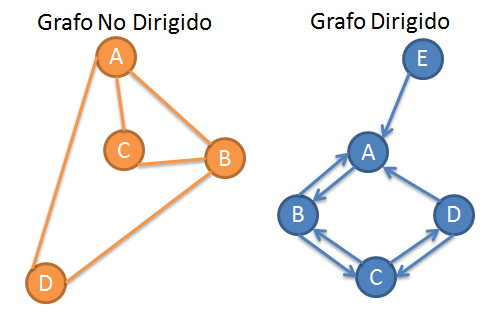
\includegraphics[width=10cm]{./Imagenes/grafo.png}
\caption{Representación gráfica de grafos.}
\label{rg6}
\end{center}
\end{figure}
\vspace*{-0.4in}

\section{Conclusiones}
Las bases de datos son un elemento fundamental en el entorno informático hoy en dí­a y tienen aplicación en la práctica totalidad de campos. Los datos son cada dí­a más voluminosos, debido no solo a una mayor cantidad de información, sino también a una mayor precisión en esta, la cual implica un mayor volumen de datos.
Las estructuras de datos son una colección de datos cuya organización se caracteriza por las funciones de acceso que se usan para almacenar y acceder a elementos individuales de datos. 

\section{Recomendaciones}
Principalmente vemos la necesidad de conocer cada dí­a más el entorno de las bases de datos. Aprender de manera didáctica y autodidacta con mayor dedicación.
Es necesario conocer que la implementación del código debe estar bien estructurado para evitar algunas redundancias innecesarias.
Conocer las especificaciones que nos presenta cuando estructuramos las tablas de cada base de datos, realizando nuestro trabajo más práctico y sencillo

\begin{thebibliography}{XXX0000}
\bibitem{PEO2019} Pulido Romero, E. Escobar Domí­nguez, Ó. y Núñez Pérez, J. Á.  (2019). Base de datos. Grupo Editorial Patria. \\https://elibro.net/es/lc/bibliotecaupt/titulos/121283

\bibitem{JOY2005} Joyanes Aguilar, L. (2005). Estructuras de datos en C. Aravaca (Madrid), Spain: McGraw-Hill Espa ña. \\https://elibro.net/es/lc/bibliotecaupt/titulos/50068

\bibitem{ZOH2008} Zohonero Martí­nez, I. y Joyanes Aguilar, L. (2008). Estructuras de datos en Java. McGraw-Hill Espa ña. \\://elibro.net/es/lc/bibliotecaupt/titulos/50117

\bibitem{JEY2007} Joyanes, L. (2007). Estructura de datos en C++. McGraw-Hill Espa ña. \\https://elibro.net/es/lc/bibliotecaupt/titulos/50123

\bibitem{ROD2012} Rodrí­guez Artalejo, M. (2012). Estructuras de datos: un enfoque moderno. Editorial Complutense. \\https://elibro.net/es/lc/bibliotecaupt/titulos/62039

\bibitem{ALL2013} Allen Weiss, M. (2013). Estructuras de datos en java (4a. ed.). Pearson Educación. \\https://elibro.net/es/lc/bibliotecaupt/titulos/108459

\end{thebibliography}
\end{document}